%%%%%%%%%%%%%%%%%%%%%%%%%%%%%%%%%%%%%%%%%%%%%%%%%%%%%%%%%%%%%%%%%%%%%%%%%%%%%
%%
%% This file provides a template that can be used in concert with the
%% ohio-etd class to generate an electronic thesis or dissertation which
%% meets the formatting requirements at Ohio University.
%%
%% To use the template, copy this file (template.tex) and ohio-etd.cls into
%% the same directory and edit this template as required.  Reference
%% ohio-etd.pdf for additional instructions on using this class.
%%
%%%%%%%%%%%%%%%%%%%%%%%%%%%%%%%%%%%%%%%%%%%%%%%%%%%%%%%%%%%%%%%%%%%%%%%%%%%%%


%% Load the class. Available options are: numbered, pdftex, cmfont,
%% singlespacetables, draft, 11pt, 12pt, leqno, and fleqn

%% ===========================================================================
%% ACCESSIBLE (TAGGED) PDF -- required for figure alt text
%% ---------------------------------------------------------------------------
%% \TaggedPDFtrue  (default): tagged PDF. Every figure carries the alt text
%%                   given with \includegraphics[alt={...}]{...}; headings,
%%                   lists, tables, links, formulas and the language are tagged,
%%                   so Acrobat's accessibility checks for them pass. Submit this.
%% \TaggedPDFfalse : untagged PDF (faster drafts). Acrobat's "Figures alternate
%%                   text" check always FAILS on an untagged PDF.
%% Compile with LuaLaTeX (Overleaf: Menu > Settings > Compiler > LuaLaTeX,
%% TeX Live 2025 or newer); pdfLaTeX also works. A tagged build needs more than
%% the 10 s Overleaf's FREE plan allows: build it locally (make) or on a plan
%% with a longer compile timeout. See README.md.
%% This block must stay ABOVE \documentclass.
%% ===========================================================================
\newif\ifTaggedPDF
\TaggedPDFtrue    % <-- true: accessible build with alt text (default); false: fast drafts
\ifTaggedPDF
  \DocumentMetadata{
    lang       = en-US,
    pdfversion = 1.7,
    tagging    = on,
  }
\else
  \DocumentMetadata{
    lang       = en-US,
    pdfversion = 1.7,
  }
\fi
\documentclass[numbered]{ohio-etd} % (no "pdftex" option: PDF output is detected automatically)

% unicode to text mapping (for accessibility test); needed for the Type 1
% fonts (all fonts under pdfLaTeX, the math fonts under LuaLaTeX)
\ifdefined\pdfgentounicode        % pdfLaTeX
  \input{glyphtounicode}\pdfgentounicode=1
\else\ifdefined\pdfvariable       % LuaLaTeX
  {\ifdefined\pdfglyphtounicode\else % (older LuaLaTeX formats)
     \def\pdfglyphtounicode{\pdfextension glyphtounicode }\fi
   \input{glyphtounicode}}\pdfvariable gentounicode=1
\fi\fi

%% Other packages that may be of use.  Delete or comment out (using a
%% percent sign in the first column) if they are not desired.  Reference
%% the corresponding documentation for more information on how to use these
%% packages.

\usepackage[square,sort&compress,numbers]{natbib} % Provides formatting for
                                                  % citations
\usepackage{textcomp} % Provides math symbols that can be used in text mode
\usepackage{amssymb}  % Provides additional AMS math symbols.  Note that
                      % amsmath is loaded as part of the ohio-etd class
\usepackage{bm}       % Provides bold-faced math symbols
\usepackage{booktabs} % Provides improved table formatting
\usepackage{comment}
\usepackage{float}
\usepackage{rotating} % for rotating table

\usepackage{ragged2e}
\usepackage{microtype}

% \usepackage{hyperref}   % comment out; ohio-etd.cls already loads it
\usepackage{xurl}
%\usepackage[normalem]{ulem}

\usepackage{xcolor}
\usepackage{wasysym}

%%%%%%%%%%%%%%%%%%%%%%%%%%%%%%%%%%%%%%%%%%%%%%%%%%%%%%%%%%%%%%%%%%%%%%
% For subfigures only (minimal interference with ohio-etd)
% this might invoke warning on compilation so should use carefully
% \usepackage{caption}
% \captionsetup{compatibility=false}
% \usepackage{subcaption}
% % Optional: ensure only subcaptions get any settings (leave normal captions alone)
% \captionsetup[sub]{}
%%%%%%%%%%%%%%%%%%%%%%%%%%%%%%%%%%%%%%%%%%%%%%%%%%%%%%%%%%%%%%%%%%%%%%
\usepackage{pdfpages}
\usepackage{import}   % helps with folders
\usepackage{dcolumn}  % Provides table columns aligned at decimal points
\usepackage{multirow} % Provides table elements spanning multiple rows
\usepackage{graphicx} % Standard package to incorporate graphics
\usepackage{embedfigurefonts} % Embeds ALL fonts used inside PDF/EPS figures
                              % (ROOT, matplotlib, gnuplot, ...), as required
                              % by TAD. Needs shell escape: automatic on
                              % Overleaf; locally compile with
                              %   lualatex -shell-escape main.tex
                              % Options and details: embedfigurefonts.sty
\usepackage{enumitem}
\usepackage[printonlyused]{acronym} % Provides a method for incorporating
                                    % acronyms and building an acronym list

\graphicspath{{figures/}} % Allows graphics files to be stored in a
                          % separate directory

%% Required front matter definitions

\degree    {PhD}              % MS, MA, MCTP, or PhD
\graduation{August}{2026}    % May, August, or December 

\title{Measurement of \texorpdfstring{$\pi^{0}$}{pi0} and \texorpdfstring{$\eta$}{eta} Meson Production in \texorpdfstring{$p+p$}{p+p} Collisions at \texorpdfstring{$\sqrt{s} = 200~\mathrm{GeV}$}{sqrt(sNN) = 200 GeV} With sPHENIX}


\author    {Sijan}{Regmi}

% this is to pass accessibility test in adobe acrobat (pro)
% the pdf title is title of thesis (and not in latex)
% pdf author is the author of the thesis
% others will remain same as this (unless if there is any change(s) needed)

\hypersetup{
    pdftitle={Measurement of pi0 and eta Meson Production in p+p Collisions at sqrt(sNN) = 200 GeV With sPHENIX},
    pdfauthor={Sijan Regmi},
    pdflang={en-US},
    pdfdisplaydoctitle=true
}

\advisor   {Justin E. Frantz}{Associate Professor, Physics and Astronomy Department}
\dean      {Matthew Ando}{Dean, College of Arts and Sciences}

\program   {Physics}            % e.g. Electrical Engineering
\department{Department of Physics and Astronomy} % e.g. School of Electrical Engineering 
                                     %      and Computer Science
\college   {College of Arts and Sciences}   % e.g. Russ College of Engineering and
                                     %      Technology
\justifying
%\abstract{Insert your abstract here}
\abstract{
This dissertation presents a study of neutral meson production in proton-proton ($p+p$) collisions at $\sqrt{s}$ = 200 \ac{GeV} collected by newly built \ac{sPHENIX} detector. \ac{sPHENIX} detector, within \ac{RHIC} facility, is a state-of-the-art successor to \ac{PHENIX} with extended pseudorapidity ($\eta$) and complete $\phi$-coverage. Our research focuses on the measurement of invariant cross section of $\eta$ meson and $\pi^{0}$ via their two-photon decay mode. The final results are compared with results from \ac{PHENIX} experiment to provide the initial validation of data measured by \ac{sPHENIX} detector. In particular, a first full physics measurement of the ratio of $\eta$ meson to $\pi^0$ production cross sections is made and found to be in good agreement with past \ac{PHENIX} measurement. 

Furthermore, this dissertation reports various background reconstruction strategies and the application of supervised machine learning to isolate $\eta$ meson signals from background. Ultimately, we discuss the implementation of calibration methods of \ac{sPHENIX} \ac{EMCal} using $\pi^0$ decaying to two photons, as well as the methods' development and validation.
% <-- IMPORTANT: keep this as the last line and no space above this line to keep everything in frontmatter otherwise we might get an error}

%% Optional front matter definitions.  Delete or comment out if not needed

%\coadvisor {Coadvisor's Full Name}{Coadvisor's Full Title}

\dedication{% vertically centered, italic
\vspace*{\fill}
\begin{center}\itshape
Dedicated to the perseverance that outlasted every setback, the discipline that prevailed over every distraction, and the countless sleepless nights that illuminated this journey marked by curiosity, resilience, and growth.


\end{center}
\vspace*{\fill}}

%\acknowledgments{Insert your acknowledgments here or comment out this line.}
%% If you prefer to provide "acknowledgements" instead (note the added "e"
%% between the "g" and the "m") then add the "e" in the macro name so that
%% it reads "\acknowledgements".}

\acknowledgements{
Several AI tools proved to be valuable, especially during the last few years of this journey. The most significant were Notebook LM (for reading papers), Google Colaboratory (Python computing), Google Gemini (for image and video generation), Perplexity AI (as a search engine), and last but not least ``ChatGPT'', which was the master of all.


Finally, I am forever grateful to the city of Athens, which has been my ``home-away-from-home'' for the past seven years. I would also like to remember NEPSA, ISU, ISSS (especially to ISSS director Diane Cahill), SAC, and HAPCAP for providing me with volunteering opportunities in different positions. Such experiences played a significant role in my personal growth. Upon leaving Athens, I realize that I am profoundly different from the person who first arrived here in 2019. And yeah, coming from Nepal, the ``mountains'' around Athens are basically adorable little speed bumps \textcolor{orange}{\smiley}.
}


%% Additional "lists" can be added to the end of the front matter using the
%% \addlistof macro.  For example:
\addlistof{Symbols}{\tagpdfsetup{table/header-rows={},table/header-columns={1}}% symbol column = row headers
\begin{tabular}{@{}ll@{}}
$\alpha$ &energy asymmetry\\
$\alpha_s$   & strong coupling constant\\
$\chi^2$   & shower shape variable \\
$\Delta R$   & angular separation in $\eta$--$\phi$ space\\
$\epsilon$   & detector efficiency\\
$\eta$   & pseudorapidity\\
$\eta$ meson   & eta meson\\
$\gamma$   & photon\\
$\Lambda_{\mathrm{QCD}}$   & QCD scale parameter\\
$\phi$   & azimuthal angle\\
$\pi^0$   & neutral pion\\
$\sqrt{s}$   & proton-proton center-of-mass energy\\
$\sqrt{s_{\mathrm{NN}}}$   & nucleon-nucleon center-of-mass energy\\
$\theta$   & polar angle\\
$\theta_{\gamma\gamma}$   & opening angle\\
$A$   & detector acceptance\\
$m_{\gamma\gamma}$   & di-photon invariant mass\\
$mrad$   & milliradian\\
$p_T$   & transverse momentum\\
$Q$   & momentum transfer\\
$z_{\mathrm{vtx}}$   & z - component of collision vertex\\
\end{tabular}
% <-- IMPORTANT: keep this as the last line and no space above this line to keep everything in frontmatter otherwise we might get an error}
%% Note that the command "\input{symbols}" can be used if the symbol list is
%% contained in a separate file called "symbols.tex"}

%\addlistof{Acronyms}{Insert your list of acronyms here or comment out this line}
\addlistof{Acronyms}{\begin{acronym}[HTTPS] % longest label for alignment
  \setlength\itemsep{0pt}
  \setlength\parskip{0pt}

    \acro{AGS}{\textbf{A}lternating \textbf{G}radient \textbf{S}ynchrotron}

    \acro{ALICE}{\textbf{A} \textbf{L}arge \textbf{I}on \textbf{C}ollider \textbf{E}xperiment}

    \acro{ATLAS}{\textbf{A} \textbf{T}oroidal \textbf{L}HC \textbf{A}pparatu\textbf{S}}

    \acro{AUC}{\textbf{A}rea \textbf{U}nder \textbf{C}urve}
    
    \acro{BNL}{\textbf{B}rookhaven \textbf{N}ational \textbf{L}aboratory}

    \acro{CMS}{\textbf{C}ompact \textbf{M}uon \textbf{S}olenoid}
    
    \acro{CNM}{\textbf{C}old \textbf{N}uclear \textbf{M}atter}

    \acro{DAQ}{\textbf{D}ata \textbf{A}cquisition}

    \acro{DoE}{\textbf{D}epartment \textbf{o}f \textbf{E}nergy}
    
    \acro{EBIS}{\textbf{E}lectron \textbf{B}eam \textbf{I}on \textbf{S}ource}
    
    \acro{EMC}{\textbf{E}uropean \textbf{M}uon \textbf{C}ollaboration}
    
    \acro{EMCal}{\textbf{E}lectro\textbf{M}agnetic \textbf{Cal}orimeter}

    \acro{FF}{\textbf{F}ragmentation \textbf{F}unction}
    
    \acro{FPGA}{\textbf{F}ield \textbf{P}rogrammable \textbf{G}ate \textbf{A}rray}
    
    \acro{GeV}{\textbf{G}iga \textbf{E}lectron \textbf{V}olt}
    
    \acro{HCal}{\textbf{H}adronic \textbf{Cal}orimeter}
    
    \acro{INTT}{\textbf{INT}ermediate Silicon \textbf{T}racker}
    
    \acro{IR}{\textbf{I}nteracting \textbf{R}egion}
    
    \acro{keV}{\textbf{k}ilo \textbf{e}lectron \textbf{V}olt}
    
    \acro{LHC}{\textbf{L}arge \textbf{H}adron \textbf{C}ollider}
    
    \acro{LHCb}{\textbf{L}arge \textbf{H}adron \textbf{C}ollider \textbf{b}eauty experiment}
    
    \acro{LINAC}{\textbf{LIN}ear \textbf{AC}celerator}
    
    \acro{MB}{\textbf{M}inimum \textbf{B}ias}
    
    \acro{MBD}{\textbf{M}in \textbf{B}ias \textbf{D}etector}

    \acro{MeV}{\textbf{M}ega \textbf{e}lectron \textbf{V}olt}

    \acro{MIP}{\textbf{M}inimum \textbf{I}onizing \textbf{P}article}
    
    \acro{MVTX}{\textbf{M}onolithic Active Pixel Sensors \textbf{V}er\textbf{T}e \textbf{X}Detector}

    \acro{NLO}{\textbf{N}ext to \textbf{L}eading \textbf{O}rder}
    
    \acro{OPPIS}{\textbf{O}ptically \textbf{P}umped \textbf{P}olarized \textbf{I}on \textbf{S}ource}
    
    \acro{PDF}{\textbf{P}arton \textbf{D}istribution \textbf{F}unction}
    
    \acro{PHENIX}{\textbf{P}ioneering \textbf{H}igh \textbf{E}nergy \textbf{N}uclear \textbf{I}nteraction e\textbf{X}periment}
    
    \acro{pp}{\textbf{p}roton - \textbf{p}roton}
    
    \acro{pQCD}{\textbf{p}erturbative \textbf{Q}uantum \textbf{C}hromo\textbf{D}ynamics}

    \acro{QA}{\textbf{Q}uality \textbf{A}ssurance}
    
    \acro{QCD}{\textbf{Q}uantum \textbf{C}hromo\textbf{D}ynamics}
    
    \acro{QED}{\textbf{Q}uantum \textbf{E}lectro\textbf{D}ynamics}
    
    \acro{QGP}{\textbf{Q}uark \textbf{G}luon \textbf{P}lasma}
    
    \acro{RF}{\textbf{R}adio \textbf{F}requency}
    
    \acro{RHIC}{\textbf{R}elativistic \textbf{H}eavy \textbf{I}on \textbf{C}ollider}

    \acro{ROC}{\textbf{R}eceiver \textbf{O}perating \textbf{C}haracteristic} 

    \acro{sEPD}{\textbf{s}PHENIX \textbf{E}vent \textbf{P}lane \textbf{D}etector}
    
    \acro{SiPM}{\textbf{Si}licon \textbf{P}hoto\textbf{M}ultiplier}

    \acro{SMD}{\textbf{S}hower \textbf{M}aximum \textbf{D}etector}
        
    \acro{sPHENIX}{\textbf{s}uper \textbf{P}ioneering \textbf{H}igh \textbf{E}nergy \textbf{N}uclear \textbf{I}nteraction e\textbf{X}periment}

    \acro{SPS}{\textbf{S}uper \textbf{P}roton \textbf{S}ynchrotron}

    \acro{STAR}{\textbf{S}olenoidal \textbf{T}racker \textbf{A}t \textbf{R}HIC}

    \acro{TeV}{\textbf{T}era \textbf{e}lectron \textbf{V}olt}
    
    \acro{TPC}{\textbf{T}ime \textbf{P}rojection \textbf{C}hamber}
    
    \acro{TPOT}{\textbf{TP}C \textbf{O}uter \textbf{T}racker}

    \acro{XGBoost}{e\textbf{X}treme \textbf{G}radient \textbf{Boost}ing}
    
    \acro{ZDC}{\textbf{Z}ero \textbf{D}egree \textbf{C}alorimeter}
    
\end{acronym}
% <-- IMPORTANT: keep this as the last line and no space above this line to keep everything in frontmatter otherwise we might get an error}

%% Use "\input{acronyms}" if the acronym list is in a separate file called
%% "acronyms.tex".  Note that the formatting generated by the acronym package
%% can be forced into singlespaced text by inserting "\setlength\itemsep{0pt}
%% \setlength\parskip{0pt}" into the "acronym" environment.} 


%% For documents created by government employees as part of their
%% employment.  The wording of the disclaimer can be specified using an
%% option.  See the documentation for more information.

% \govtdisclaimer    

% \notables  % Prevent a list of tables from being created
% \nofigures % Prevent a list of figures from being created

\setcounter{tocdepth}{2}
\begin{document}

\makefrontmatter    % Creates all of the front matter pages.

%% Body of the text follows, using \chapter, \section, \subsection,
%% \subsubsection, \paragraph, and \subparagraph to generate the
%% section headings.  For convenience, it may be useful to break the
%% full document into separate files, perhaps divided by chapters.  In
%% that case, the files would be loaded here using "\input{filename}"


% === Chapter 1 ===
\chapter{Introduction and Physics Motivation}
\import{Thesis/1_Intro_and_Motivation/}{1_1_PhysicsVariable.tex}


% === Chapter 2 ===
\chapter{Theoretical Framework}
\import{Thesis/2_Theoretical_Framework/}{2_1_QCD_Overview.tex}


% === Chapter 3 ===
\chapter{Experimental Setup}
\import{Thesis/3_Experimental_Setup/}{3_1_RHIC_Facility.tex}


% === Chapter 4 ===
\chapter{Electromagnetic Calorimeter Calibration}
\import{Thesis/4_EMCal_Calibration/}{4_1_EMCal_Calibration.tex}


% === Chapter 5 ===
\chapter {Neutral Meson Analysis}
\import{Thesis/5_Analysis_Methods/}{5_1_EventDataSelect.tex}


% === Chapter 6 ===
\chapter{Results}
\import{Thesis/6_Results/}{6_1_InvMassSpectra.tex}


% === Chapter 7 ===
\chapter{Discussion and Conclusion}
\import{Thesis/7_Discussion_and_Conclusion/}{7_1_Result_Summary.tex}


\references{

  % ---------------------------------------------------------
  % References only:
  % URLs and DOIs = blue + clickable + underlined
  % ---------------------------------------------------------

  \hypersetup{
    pdfborder={0 0 1},
    pdfborderstyle={/S/U/W 1},
    urlbordercolor=blue
  }

  % Website URLs:
  % blue text; xurl handles line breaking
  \renewcommand\UrlFont{\color{blue}\normalfont}

  % DOI links produced by alphaurl_etd.bst:
  % make the visible DOI text blue
  \let\oldhref\href
  \renewcommand{\href}[2]{%
    \oldhref{#1}{\textcolor{blue}{#2}}%
  }

  \bibliographystyle{alphaurl_etd}
  \bibliography{references.bib}
}


\appendix  % Indicates the transition from chapters to appendices.


\chapter{Run 24 \texorpdfstring{$p+p$}{pp} Data Set: Selected Runs}
\label{app:runs}

The following run numbers corresponding to the Run 24 $p+p$ data set were used in this analysis. These runs were selected from golden run list available and corresponds to zero crossing angle. Following full run list is provided for reproducibility.

\begin{small}
\begin{flushleft}

47289,
47291,
47293,
47306,
47310,
47313,
47314,
47315,
47316,
47333,
47334,
47357,
47360,
47363,
47376,
47377,
47378,
47379,
47380,
47381,
47382,
47391,
47393,
47394,
47395,
47396,
47440,
47443,
47454,
47455,
47457,
47458,
47459,
47461,
47462,
47463,
47464,
47474,
47478,
47480,
47481,
47482,
47484,
47485,
47489,
47491,
47492,
47494,
47495,
47497,
47501,
47502,
47503,
47505,
47506,
47507,
47509,
47513,
47514,
47516,
47517,
47519,
47521,
47522,
47524,
47525,
47540,
47547,
47548,
47549,
47552,
47557,
47568,
47634,
47635,
47636,
47637,
47638,
47650,
47657,
47658,
47659,
47661,
47662,
47664,
47666,
47667,
47714,
47715,
47716,
47719,
47720,
47721,
47722,
47723,
47724,
47725,
47726,
47727,
47729,
47730,
47732,
47733,
47783,
47831,
47834,
47889,
47890,
47892,
47893,
47940,
47944,
47946,
47966,
47972,
47973,
47975,
47976,
47977,
47978,
47979,
47982,
47998,
47999,
48001,
48002,
48008,
48073,
48076,
48079,
48082,
48084,
48085,
48086,
48088,
48089,
48097,
48099,
48166,
48172,
48176,
48177,
48179,
48181,
48185,
48230,
48233,
48638,
48639,
48640,
48645,
48656,
48657,
48658,
48660,
48701,
48706,
48720,
48721,
48722,
48725,
48726,
48727,
48730,
48731,
48732,
48734,
48735,
48736,
48742,
48743,
48745,
48746,
48801,
48803,
48805,
48806,
48807,
48810,
48811,
48812,
48813,
48814,
48824,
48826,
48828,
48829,
48830,
48832,
48836,
48838,
48839,
48863,
48864,
48865,
48867,
48883,
48884,
48885,
48888,
48891,
48892,
48893,
48894,
48895,
48897,
48899,
48900,
48901,
48902,
48903,
48935,
48938,
48940,
48943,
48946,
48947,
48949,
48951,
48952,
48971,
48976,
48982,
48983,
48984,
48985,
48986,
48987,
48988,
48989,
48990,
48991,
49019,
49026,
49027,
49029,
49030,
49031,
49057,
49059,
49060,
49061,
49062,
49063,
49064,
49065,
49066,
49067,
49068,
49069,
49070,
49071,
49072,
49073,
49098,
49099,
49100,
49110,
49111,
49113,
49114,
49116,
49117,
49118,
49121,
49125,
49126,
49127,
49128,
49132,
49133,
49134,
49135,
49136,
49137,
49138,
49139,
49140,
49141,
49142,
49143,
49144,
49155,
49157,
49158,
49159,
49165,
49168,
49217,
49218,
49219,
49224,
49226,
49227,
49228,
49229,
49230,
49232,
49233,
49240,
49241,
49244,
49245,
49246,
49247,
49248,
49249,
49250,
49251,
49253,
49254,
49262,
49263,
49264,
49265,
49266,
49267,
49268,
49270,
49307,
49308,
49309,
49310,
49311,
49312,
49313,
49314,
49316,
49317,
49324,
49329,
49330,
49331,
49332,
49337,
49339,
49340,
49341,
49342,
49345,
49346,
49347,
49348,
49349,
49351,
49352,
49353,
49356,
49358,
49359,
49360,
49361,
49362,
49365,
49366,
49367,
49368,
49369,
49373,
49374,
49376,
49377,
49378,
49379,
49380,
49381,
49382,
49383,
49384,
49385,
49389,
49390,
49432,
49433,
49434,
49435,
49437,
49438,
49439,
49440,
49445,
49446,
49447,
49448,
49449,
49451,
49452,
49453,
49454,
49455,
49456,
49457,
49464,
49466,
49468,
49652,
49653,
49655,
49656,
49657,
49658,
49659,
49660,
49661,
49662,
49664,
49665,
49666,
49736,
49737,
49742,
49743,
49749,
49751,
49752,
49756,
49758,
49760,
49761,
49762,
49763,
49910,
49914,
49919,
49921,
49922,
49923,
49925,
49926,
49928,
49929,
49930,
49932,
49934,
49959,
49960,
49961,
49962,
49964,
49965,
49966,
49967,
49968,
49969,
49970,
50033,
50034,
50036,
50045,
50046,
50047,
50048,
50067,
50068,
50070,
50073,
50074,
50075,
50076,
50077,
50343,
50376,
50377,
50380,
50463,
50464,
50465,
50466,
50467,
50468,
50470,
50471,
50483,
50491,
50492,
50493,
50496,
50497,
50500,
50501,
50517,
50520,
50522,
50526,
50527,
50528,
50529,
50530,
50531,
50535,
50536,
50545,
50546,
50548,
50549,
50550,
50551,
50552,
50553,
50554,
50558,
50560,
50561,
50562,
50563,
50564,
50565,
50569,
50570,
50596,
50597,
50598,
50599,
50600,
50601,
50602,
50603,
50604,
50605,
50606,
50607,
50613,
50614,
50615,
50616,
50617,
50650,
50654,
50655,
50656,
50658,
50660,
50661,
50662,
50663,
50664,
50665,
50666,
50667,
50668,
50669,
50670,
50671,
50672,
50673,
50674,
50675,
50676,
50677,
50678,
50679,
50853,
50854,
50857,
50862,
50863,
50874,
50875,
50876,
50885,
50886,
50887,
50889,
50897,
51015,
51093,
51152,
51154,
51159,
51160,
51162,
51163,
51165,
51166,
51167,
51171,
51172,
51175,
51176,
51177,
51178,
51179,
51180,
51181,
51182,
51183,
51187,
51188,
51200,
51201,
51202,
51206,
51208,
51209,
51210,
51211,
51212,
51213,
51214,
51215,
51217,
51220,
51222,
51225,
51226,
51228,
51229,
51230,
51234,
51236,
51237

\end{flushleft}
\end{small}

\chapter{External Photon Conversion in sPHENIX Detector}
\label{app:external_conversion}

\section{Overview of External Conversion}

In heavy ion collision, precision of \ac{EMCal} measurements relies on the accurate reconstruction of photons originating from the primary collision vertex. However, before reaching the \ac{EMCal}, these photons must traverse the internal detector subsystems like \ac{MVTX}, \ac{INTT}, \ac{TPC} and the beryllium beam pipe. These subsystems and their mechanical support structures represent a significant material budget. Any photon traversing this material possess a non-negligible probability of undergoing pair production ($\gamma \rightarrow e^+ + e^-$) before interacting with the \ac{EMCal}. In addition, the \ac{sPHENIX} detector operates within a 1.4~T (Tesla) magnetic field which deflects those converted $e^+ e^-$ pairs significantly. Such deflection, sometimes, can create two distinct and well separated \ac{EMCal} clusters. Since, external conversion affects the clusters, they should be corrected accounted for our study of neutral mesons.

\section{Neutral Meson Reconstruction}

As we analyzed neutral meson via two photon decay mode, we expect two \ac{EMCal} clusters: one for each photon. As external conversion of photon creates more than two clusters, thus, introduces a systematic effect in our analysis. The most robust way of analyzing external conversion utilized the track related information. Since such information were not available for our data, we estimated the external conversion via the number of \ac{EMCal} clusters in simulation. For this, we simulated single meson decay per event and pass through the full \textbf{GEANT4} description of the \ac{sPHENIX} detector. In reconstructed data, if there exists more than two clusters, those meson certainly have undergone external conversion. If only one cluster is present, we ignore that meson in our analysis, as they could be associated with efficiency and not external conversion.

The situation becomes nontrivial when exactly two clusters were present. To study this subtle situation, we developed a conservative method to identify if either of the photon from parent meson have converted after interacting with detector. First, we matched each cluster to one of the two truth photons by choosing the closest in $\Delta R$. Such matching must be unique in a sense there must be one photon to one cluster matching. Additional criteria was that every matches must be sufficiently close in angular distance ($\Delta R \leq 0.5$) and energy asymmetry between photon and cluster must be $E_{\alpha} \leq 0.6$. When any of these criteria was not satisfied, the parent meson was considered as suffering from external conversion. 

 

\begin{figure}[H]
  \centering
  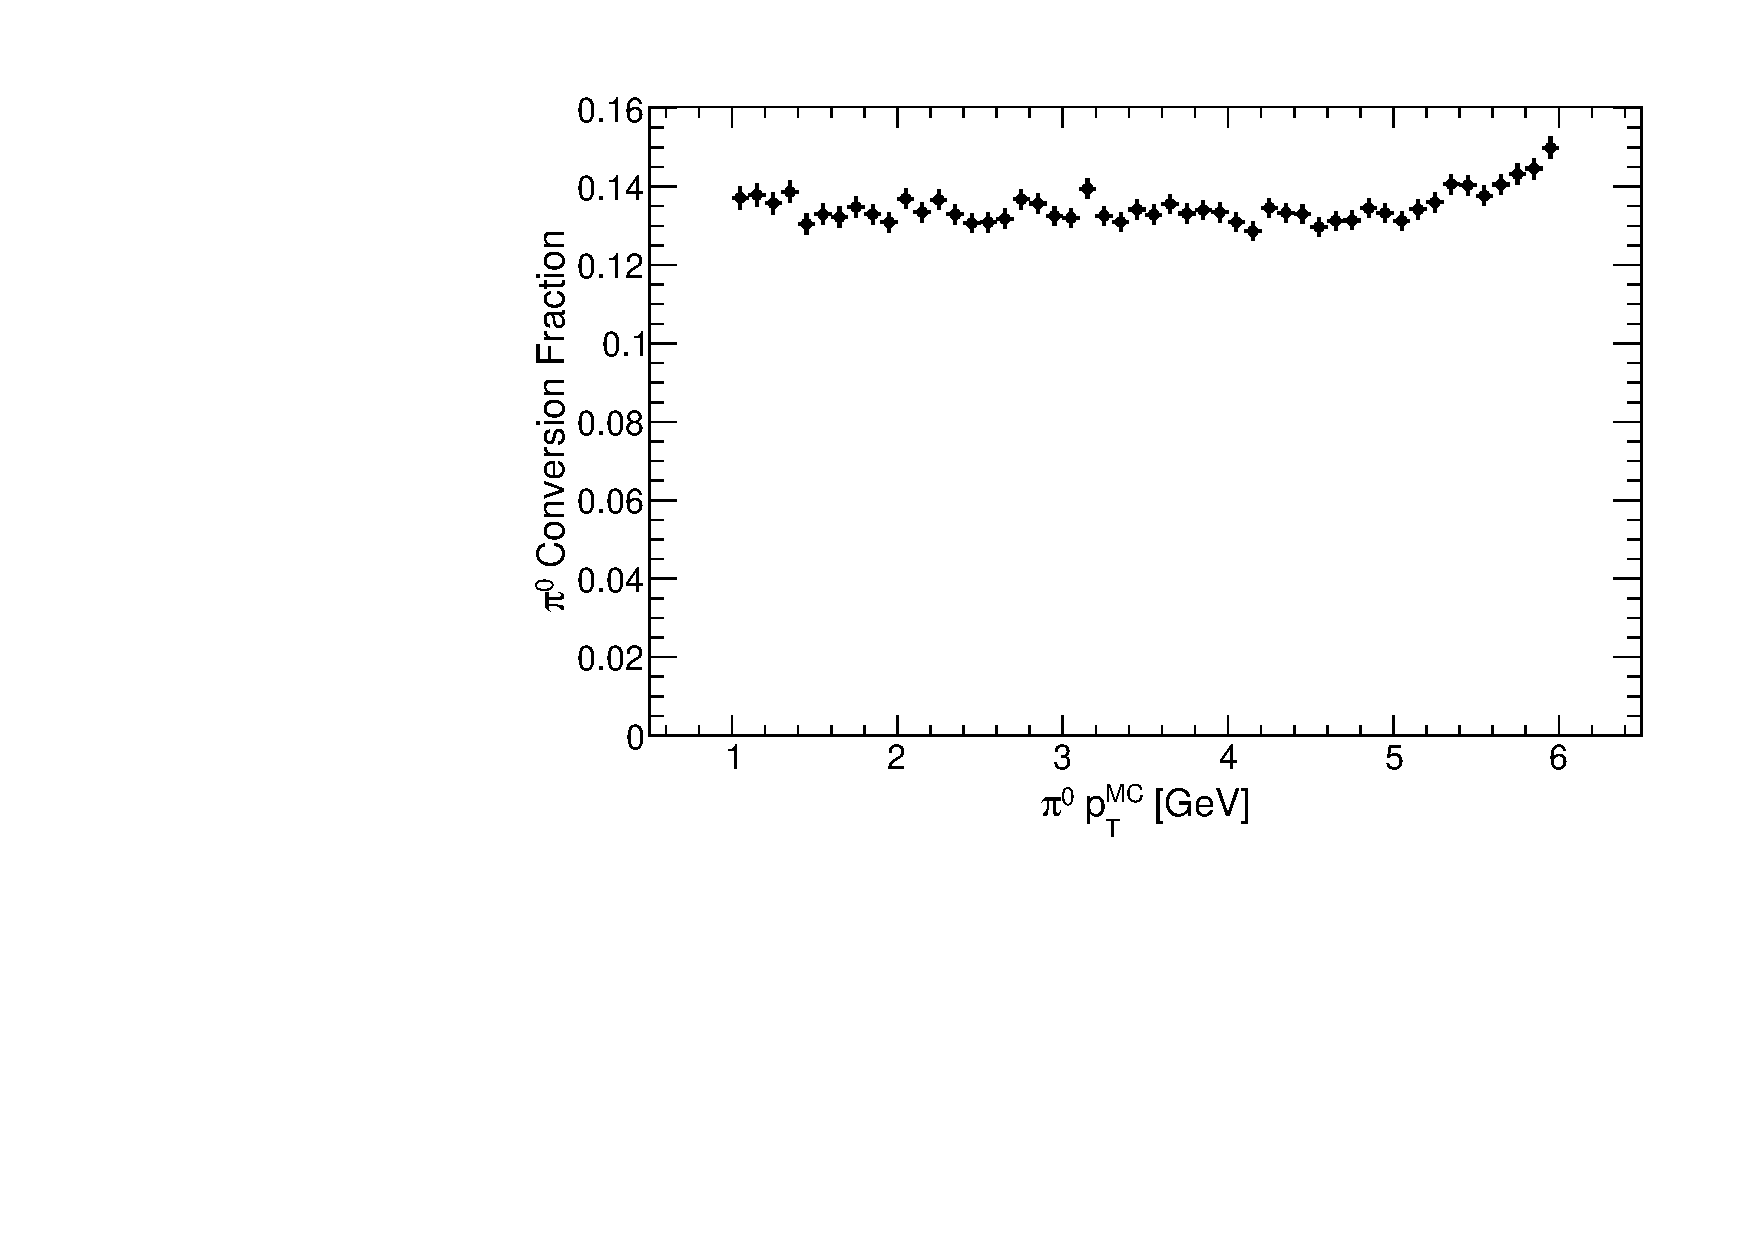
\includegraphics[width=0.95\textwidth,
    alt={Plot of the fraction of simulated neutral pions with at least one
         converted photon versus generated transverse momentum from 1 to
         6 GeV. The fraction is nearly constant at about 0.13 to
         0.14.}]{Images/App/frac_pi0_conversion.pdf}
  
  \caption{Study of external photon conversions as a function of transverse momentum ($p_T$) for $\pi^0 \rightarrow \gamma\gamma$, where at least one of the photon gets converted before being detected in \ac{EMCal}.}

  \label{fig:pi0_conver}
\end{figure}


\begin{figure}[H]
  \centering
  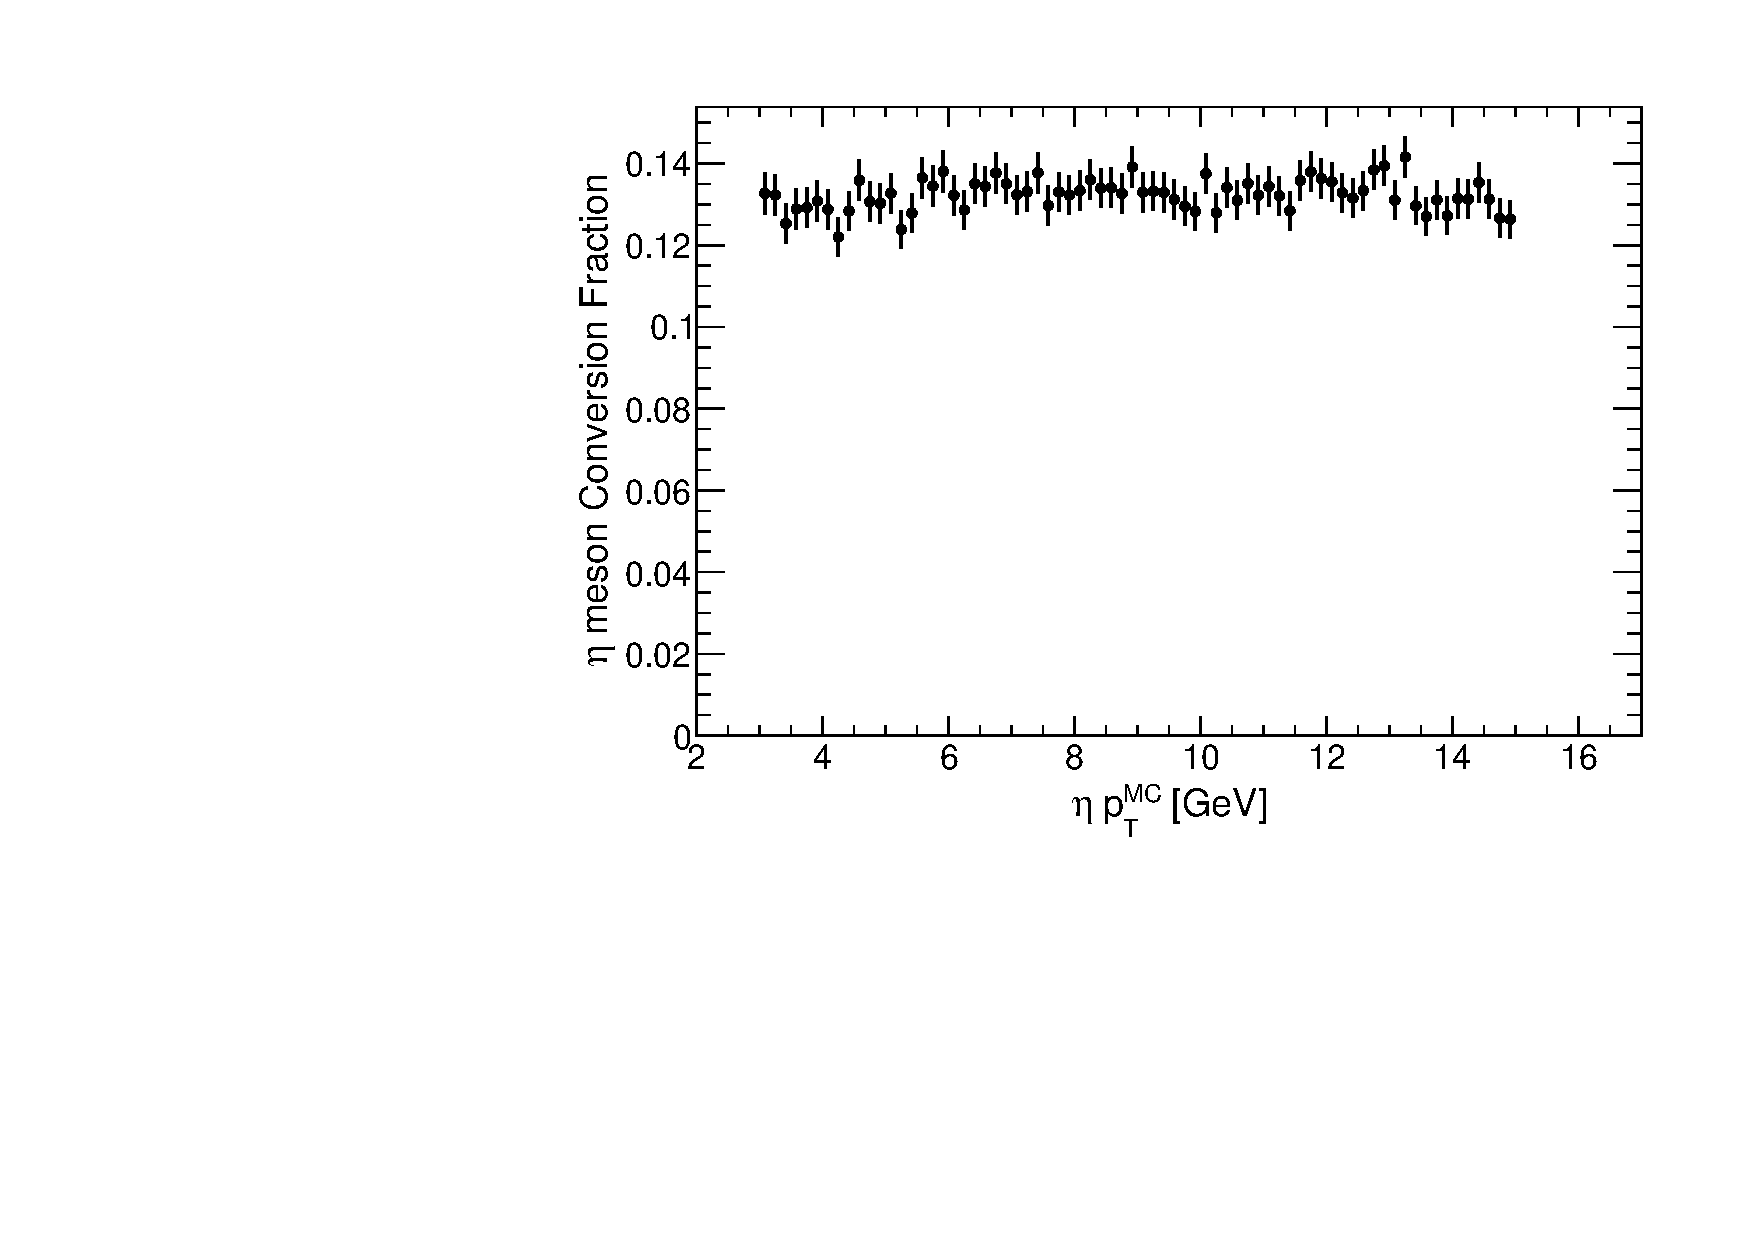
\includegraphics[width=0.95\textwidth,
    alt={Plot of the fraction of simulated eta mesons with at least one
         converted photon versus generated transverse momentum from 3 to
         15 GeV. The fraction is nearly constant at about
         0.13.}]{Images/App/frac_eta_meson_conversion.pdf}
  \caption{Study of external photon conversions as a function of transverse momentum ($p_T$) for $\eta$ meson decaying to two photons. Here, the conversion fraction reflects the probability that at least one of the decayed photon undergoes conversion.}

  \label{fig:eta_conver}
\end{figure}



The figure \ref{fig:pi0_conver} and figure \ref{fig:eta_conver} suggest approximately 13 - 14 \% of both $\pi^0$ and $\eta$ meson was affected by external conversion which is significant for our study. As this study was a simple conservative estimate, this percentage could be slightly different on using more robust analysis. This conclusion give us a motivation to use side-band fitting method as primary standard method for background estimation.
 
The external photon conversion was fully modeled within the detector simulation framework, and its impact was systematically propagated while calculating detector efficiency. Therefore, no independent or supplementary study was required to account for this effect for the scope of this study.


\chapter{Tables of Invariant Cross Section Measurements}

\begin{table}[htbp]
\centering
\normalsize
\setlength{\tabcolsep}{5pt}

\caption{The invariant cross section and its associated statistical and systematic uncertainties of $\pi^0$ as a function of transverse momentum ($p_T$), for pseudorapidity range of $-0.35 < \eta < 0.35$.}
\label{tab:inv_cross_section_pi0_PH}

\begin{tabular}{ccccc}
\hline
$p_T$ [GeV] &
Invariant Cross Section &
Stat.\ Error &
Syst.\ Error (+) &
Syst.\ Error ($-$) \\
\hline

1.713  & $8.2299\times10^{-2}$ & $0.1812\times10^{-2}$ & $6.6437\times10^{-2}$ & $3.6964\times10^{-2}$ \\
2.218  & $8.0510\times10^{-3}$ & $0.1078\times10^{-3}$ & $1.9647\times10^{-3}$ & $1.9689\times10^{-3}$ \\
2.722  & $1.8119\times10^{-3}$ & $0.0214\times10^{-3}$ & $0.4695\times10^{-3}$ & $0.5406\times10^{-3}$ \\
3.224  & $4.8312\times10^{-4}$ & $0.0572\times10^{-4}$ & $1.2116\times10^{-4}$ & $1.4783\times10^{-4}$ \\
3.727  & $1.4973\times10^{-4}$ & $0.0192\times10^{-4}$ & $0.4117\times10^{-4}$ & $0.4597\times10^{-4}$ \\
4.229  & $5.3093\times10^{-5}$ & $0.0830\times10^{-5}$ & $1.3747\times10^{-5}$ & $1.6158\times10^{-5}$ \\
4.730  & $2.2537\times10^{-5}$ & $0.0453\times10^{-5}$ & $0.5493\times10^{-5}$ & $0.6754\times10^{-5}$ \\
5.232  & $9.2706\times10^{-6}$ & $0.2674\times10^{-6}$ & $2.2252\times10^{-6}$ & $2.7923\times10^{-6}$ \\
5.733  & $4.1143\times10^{-6}$ & $0.0424\times10^{-6}$ & $0.9843\times10^{-6}$ & $1.2369\times10^{-6}$ \\
6.235  & $2.1981\times10^{-6}$ & $0.0242\times10^{-6}$ & $0.5299\times10^{-6}$ & $0.6587\times10^{-6}$ \\
6.736  & $9.9656\times10^{-7}$ & $0.1251\times10^{-7}$ & $3.3433\times10^{-7}$ & $3.2794\times10^{-7}$ \\
7.237  & $5.2737\times10^{-7}$ & $0.0789\times10^{-7}$ & $1.6349\times10^{-7}$ & $1.7722\times10^{-7}$ \\
7.738  & $3.4761\times10^{-7}$ & $0.0598\times10^{-7}$ & $0.8770\times10^{-7}$ & $1.6335\times10^{-7}$ \\

\hline
\end{tabular}
\end{table}




\end{document}
